\textbf{Beispiel 4}\\ \\
a)\\ \\
Zeichnung zur Darstellung für die Sichtfaktorberechnung:
\begin{figure}[h]
	\centering
	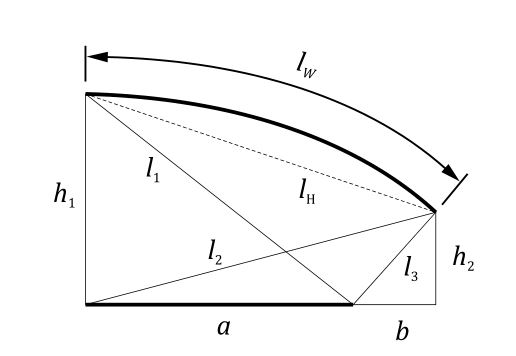
\includegraphics[width= 10cm]{tikz/27_09_2019_4a}
\end{figure}
\newline
Die dargestellten Längen lauten
\begin{align*}
	l_1 &= \sqrt{a^2 + h_1^2} \\
	l_2 &= \sqrt{(a + b)^2 + h_2^2} \\
	l_3 &= \sqrt{b^2 + h_2^2} \\
	l_H &= \sqrt{(a + b)^2 + (h_1 - h_2)^2}
\end{align*}
Der Sichfaktor von Probe zur Wand wird mittels der Cross-String-Methode bestimmt und lautet somit
\[
	F_{SW} = \frac{l_1 + l_2 - l_3 - h_1}{2a}
\]
Der anderen Sichtfaktoren die von der Probe ausgehen lautet damit
\begin{align*}
	F_{SS} &= 0 \\
	F_{SU} &= 1 - F_{SW}
\end{align*}
Die Faktoren ausgehend von der Wand lauten
\begin{align*}
	F_{WS} &= \frac{l_1 + l_2 - l_3 - h_1}{2l_W}
\end{align*}
Für die Berechnung des Faktors von der Wand auf sich selbst betrachtet man die Hilfsfläche H. Diese befindet sich dort wo in der Zeichnung $l_H$ eingezeichnet ist. Somit lautet nun dieser Sichtfaktor
\begin{align*}
	F_{H} &= 0 \\
	F_{HW} &= 1 \\
	F_{WH} &= \frac{l_H}{l_W} \\
\end{align*}
Zum besseren Verständnis stellt man eine nur zur Bestimmung dieses einen Sichtfaktors die Matrix
\[
	\textbf{F}_{extra} = \begin{bmatrix}
		F_{HH} & F_{HW} \\
		F_{WH} & F_{WW}
	\end{bmatrix}
\]
auf. Somit lauten die restlichen Sichtfaktoren der eigentlich gesuchten Matrix
\begin{align*}
	F_{WW} &= 1 - F_{WH} \\
	F_{WU} &= 1 - F_{WS} - F_{WW}
\end{align*}
b)\\ \\
Mit den Ergebnissen aus a), dem Formalismus für die Nettowärmestromdichte und den Vektoren
\begin{align*}
	\dot{\textbf{q}} &= \begin{bmatrix}
		\dot{q}S & \dot{q}_W & \dot{q}_U
	\end{bmatrix}^T \\
	\textbf{T}^4 &= \begin{bmatrix}
		T_S^4 & T_W^4 & T_U^4
	\end{bmatrix}^T \\
	\varepsilon &= \begin{bmatrix}
		\varepsilon_S & 1 & 1
	\end{bmatrix}^T
\end{align*}
lautet die Nettowärmestromdichte an der Oberseite der Probe
\[
	\dot{q}_s = \varepsilon_S\sigma\left(T_S^4 - T_W^4F_{SW} - T_U^4F_{SU}\right)
\]
c)\\ \\
Der Wärmestrom, der die Probe durchläuft lautet in Abhängigkeit von P 
\[
	\dot{q} = \frac{P_{el}}{a} = \dot{q}_S
\]
d) \\ \\
Nun werden die Ergebnisse aus b) und c) gleichgesetzt und durch umformen erhält man
\[
	T_S = \sqrt[4]{\frac{P_{el}}{a\sigma \varepsilon_S} + T_W^4F_{SW} + T_U^4F_{SU}}
\]
e)\\ \\
Aus dem Wärmeleitgesetz kann man nun die gesuchte Temperaturverteilung ermitteln. Diese lautet somit
\begin{align*}
	\dot{q} &= -\lambda(t)\frac{\text{d}T}{\text{d}y} \\
	\dot{q}\text{d}y &= -\lambda(t)\text{d}T \\
	\frac{P_{el}}{a}\int_{\tilde{y} = a}^{y}\text{d}\tilde{y} &= -C_\lambda\int_{\tilde{T} = T_S}^{T}\lambda\text{d}\tilde{T} \\
	\frac{P_{el}}{a}(y - a) &= -\frac{1}{2}C_\lambda(T^2 - T_S^2) \\
	T(y) &= \sqrt{T_S^2 - \frac{2P_{el}}{aC_\lambda}(y - a)}
\end{align*}